\subsubsection{Application}
The Application is further decomposed into two different layers
(Figure \ref{fig:sd-app-init}:
\begin{itemize}
	\item \textit{Interface Layer} - provides the remote services to Application Layer by acting as an interface
 towards the underlying layers (i.e. middleware).
	\item \textit{Application Layer} - handles the application logic.
\end{itemize}
Thus, the Application Layer communicates with
other applications transparently without knowing if they are local or remote.
This approach has been inspired by the TCP/IP and OSI models.
\\
The following sub-layers compose Interface Layer:
\begin{itemize}
	\item \textit{Session Layer} -
	handles remote connections though a TCP socket;
	\item \textit{Presentation Layer} -
	handles messages formats and conversions;
	\item \textit{Service Layer} -
	implements an event loop with a worker pool and different kind of queues
	for the requests (i.e. synchronous and asynchronous). It converts the
	requests into procedure calls by leveraging a skeleton object.
	Also, it offers the specular service through a stub object and a pipeline,
	necessary to build specific remote requests.
\end{itemize}
\subsubsection{Bootstrap}

The bootstrap process consists of two ordered and separated processes:

\begin{enumerate}
  \item \textbf{Initialization:} instantiates and configures the necessary
    resources for the application;
  \item \textbf{Activation:} starts the application.
\end{enumerate}

Clearly, the activation phase depends on initialization.
While the initialization process is automatically triggered at node creation,
this is not the case for activation, which is instead triggered by the
middleware.
Moreover, at the Application Layer level, we have to consider the dependencies
among the entity types (which are depicted in Figure
\ref{fig:sd-entity-types-deps}).

The overall bootstrap process, which mimics UNIX init \cite{online-tlsag},
is divided in two ordered parts:
\begin{enumerate}
  \item \textbf{Init:} initialize all the sublayers of each macro layer,
  following a bottom up approach (from \verb|interface_layer.session| to
  \verb|application.scheduling|).
  The initialization order is given by the fact that the upper
  layers need the services provided by the underlying layers to work
  correctly (Figure \ref{fig:sd-app-init});
  \item \textbf{Start:} IL forwards the start message sent from the
  middleware to the Application Layer.
  Therefore, this event is exclusively triggered by the middleware.
\end{enumerate}

\begin{figure}[H]
  \centering
  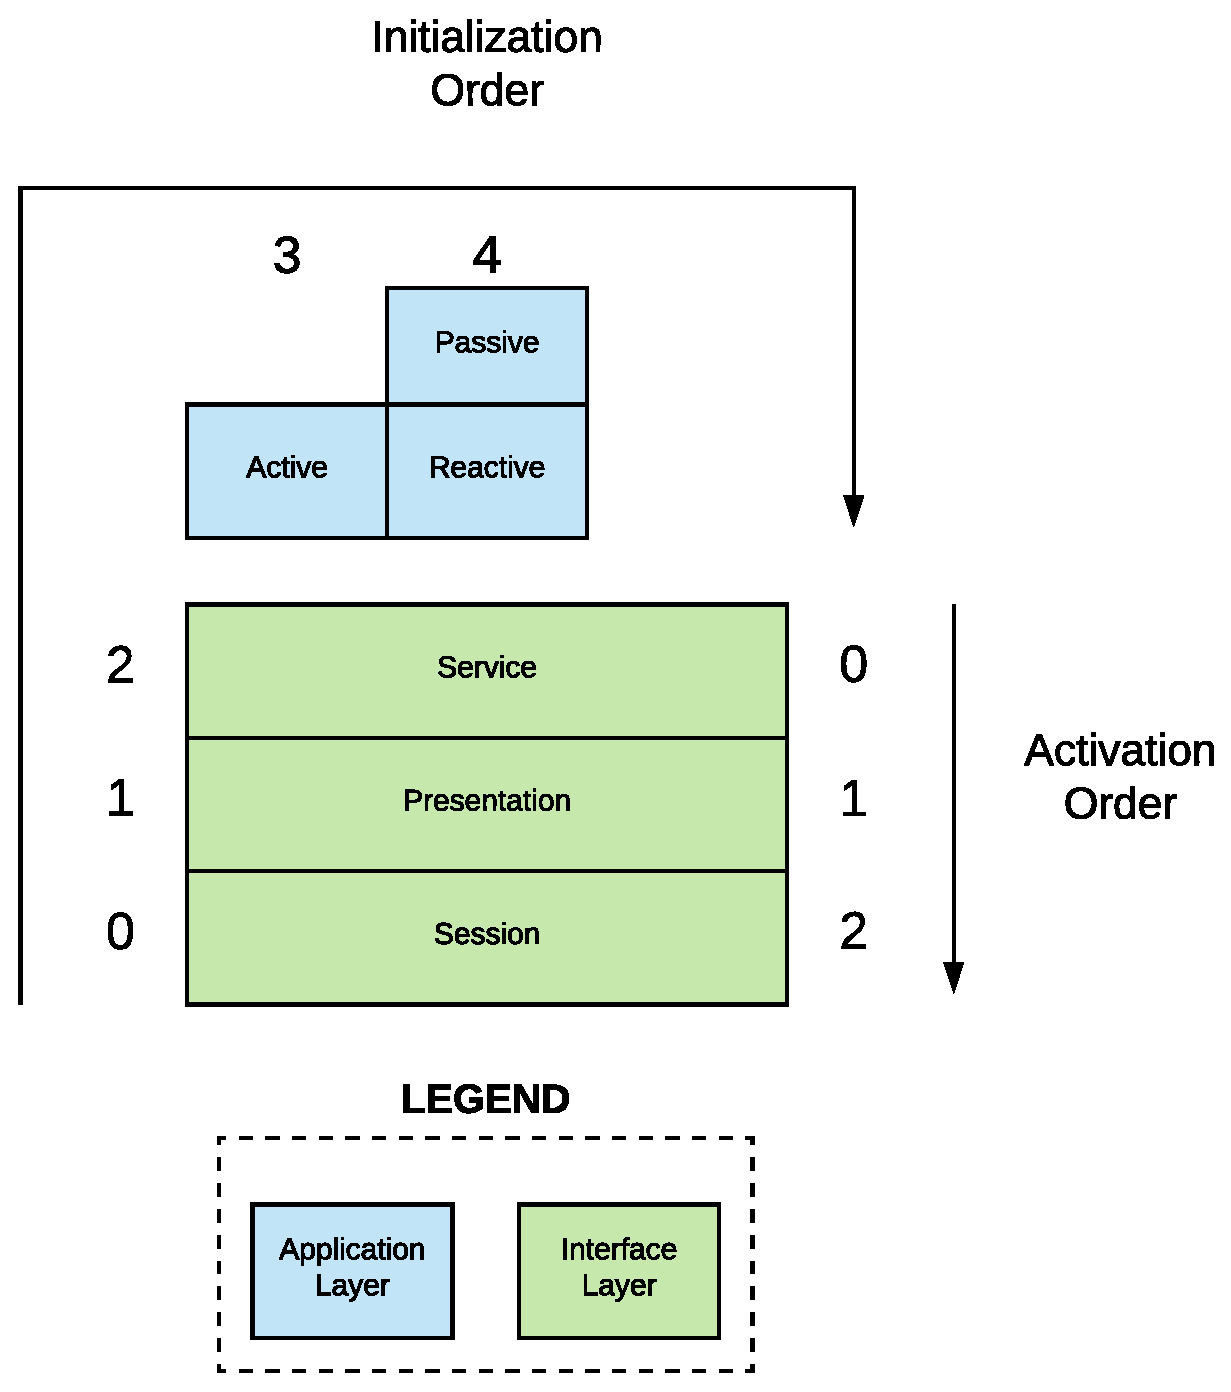
\includegraphics[scale=0.5,keepaspectratio]
    {images/solution/init_activate.eps}
  \caption{Application Bootstrap - Init}
  \label{fig:sd-app-init}
\end{figure}


\subsubsubsection{Init}

Each application node contains the \textit{Init} process,
which is the parent of all the application processes.
The execution steps of \textit{Init} are depicted in Figure
\ref{fig:sd-app-init}.
It instantiates the resources of each layer, thus making
Interface Layer and Application Layer transit from the \verb|inactive|
to the \verb|ready| state.
For example, each sublayer of Interface Layer instantiates its own pool of
LWPs\footnote{lightweight processes}.

The Application Layer initialization completes in the following order:

\begin{enumerate}
  \item \textbf{Active:} the entities which move in the city (e.g.,
    pedestrians);
  \item \textbf{Reactive:} the infrastructure of the city (e.g., streets);
\end{enumerate}

The Scheduling package, which manages the execution order for the events of the
Application Layer, does not require an initialization step. This package
will be started directly through the start message.


Since the \textit{Passive} entities are stateless and
logically belong to \textit{reactive} entities (e.g., speed limits belong to
roads), they will be instantiated along with them
(Figure \ref{fig:sd-entity-types-deps}).

When \textit{Reactive} completes its initialization, \textit{Init}
signals the Application layer completion to each sublayer of Interface Layer
in the following order:

\begin{enumerate}
  \item \textbf{Service:} provides activators and pipelines services to
    application layer;
  \item \textbf{Presentation:} provides data conversion services;
  \item \textbf{Session:} provides network connection services (e.g., senders
  and receivers).
\end{enumerate}

\textit{Init} triggers the transition of each IL sublayer state from
\verb|ready| to \verb|active|.
The activation order is extremely important to proactively avoid
message losses between remote nodes.
Indeed, at this stage, the application layer is
not able to generate or receive messages because the start message has not
been sent by the middleware. Obviously, IL is a reactive component
of the backend subystem. Thus, its \verb|active| state means
that all the workers of IL have started their event loop.
Their loop execution is triggered each time a
message arrives. Indeed, the workers are blocked on unbounded synchronized
queues which have been designed to be thread safe \cite{taft2006ada}.


The service and the presentation layer are activated before the session layer;
the latter exposes a remote communication channel through TCP
sockets.
Finally, the application is ready to communicate because both of its layers
has been activated.

Now, the Application waits the \verb|start|
message from the middleware.


A crash of the \textit{Init} process, occurring before the end of the
bootstrap, is detected by the middleware layer. The expiration
of a timeout triggers a retransmission from the middleware side.
Note that this model should also work for a bootstrap which is executed
starting
from a valid snapshot of the system, with the only difference consisting in
divergent values of the configuration file.
Indeed, for each simulation we will use a set
of configurations which is going to be different for each city.

\subsubsubsection{Start}

When \textit{Init} completes, the Application Layer is in a \verb|ready| state
while Interface Layer is in an \verb|active| state.
The first message sent by the middleware towards the Interface Layer is a
\verb|start| message which triggers the Application Layer activation.

The \verb|start| message kickoffs the scheduler, causing it to load the set
of actions declared in its configuration file. An action is a $<$\verb|agent|,
\verb|time_span|$>$ pair, i.e., the active entity \verb|agent| will act in
\verb|time_span| milliseconds.

\subsubsubsection{Termination}
When describing the shutdown of the whole system, we assumed 
the application terminates gracefully.
In this section we show the algorithm that is used to achieve this goal.

As we can see from figure \ref{fig:app-proc-tree}, the termination follows the
opposite order of the bootstrap.

\begin{enumerate}
  \item The \textit{Master} task $M$ stops active entities, e.g. pedestrians;
  \item After stopping active entities, $M$ saves their state into a file;
  \item $M$ saves into a file the state of reactive entities. 
  It is important to notice their internal state is now safetely savable, 
  since no active entities can modify it anymore;
  \item $M$ sends an \texttt{app\_shut} message to the middleware;
  \item $M$ terminates itself and the entire application consequently stops.
\end{enumerate}

The middleware layer can request the application to stop via the
\texttt{app.shutdown} call.

The last operation the \textit{Master} task does is to send a message for apprising
the middleware layer of the successful termination of the application one.
Similarly to the bootstrap phase, the middleware expects to receive this
message within a certain amount of time. 
In order to do so, when sending the message, $M$ also starts a timeout.
Wherefore if it expires before receiving a response message from the middleware layer, 
it calls again the \texttt{app.shutdown} procedure the application exposes.

\subsubsubsection{Interaction between entities}

The application contains several interactions among entities that have to be
specified in order to understand well how to approach different problems.

\paragraph{Entering a road} Moving entities enter a road by entering a stretch
that is located at the beginning of the road and that is treadable by their
specific entity type.

\paragraph{Entering a road stretch} Moving entities who want to enter a new
road stretch can do it whenever there is room for them in that stretch. In
particular, a roadway stretch can be trod for at most one vehicle at the same
time.

\paragraph{Zebra crossings} Vehicles which want to enter a road stretch that
has zebra crossings painted on it has to wait for pedestrians or bikes to free
all stretches of that particular crossing.

\paragraph{Changing roadway lane} A vehicle that is on the i-th road stretch
which wants to change lane has to check whether the (i+1)-th stretch in the
wanted direction is free.

In that case, the vehicle enters the stretch of the other lane; otherwise, if a
timeout expires before a vehicle is able to change lane, then it gives up on
it and proceeds forward to the next stretch.

\paragraph{Crossroads} Every road that is connected to a crossroads is marked
with a cardinal point (N/E/W/S). The crossroads holds all the logic necessary
for vehicles to follow the yield rules we described in
\ref{sec:pa-domain-problems}.

There could be a situation in which there is a standstill, for example when
four cars want all to go straight in a four-way crossroads. In this case, the
crossroads will make a car yield the right-of-way to another one.

Pedestrians can only walk on the corner of the crossroads, thus passing to the
adjacent piece of road (e.g. a pedestrian that is coming from the ``southern''
side of the western road can only enter the southern street on the ``western''
side).

\paragraph{Entering a building} When a moving entity is in the stretch where
there is the entrance of a building, then it may enter the building.

If the moving entity is a vehicle, it has to wait for all other entities who
are in the intermediate stretches to move away.

\paragraph{Exiting a building} When a moving entity is exiting a building, it
has to check whether there is room for her to move out.

If the entity is a vehicle, it has to yield the right-of-way to upcoming
vehicles and to wait that eventual sidewalks or bicycle path stretches in front
of the building are free too.

\paragraph{Choosing to use a vehicle} An entity $e$ who wants to leave a
building $b_e$ to a destination $d_e$ may randomly decide not to travel by
foot. She can leave only if:

\begin{itemize}
  \item the path from $b_e$ to $d_e$ does not include any destination of other
    people who are leaving from $b$ and viceversa. Otherwise, they would share
    the vehicle if there is enough room;
  \item there is an available vehicle in $b$; and
  \item the capacity of the destination building $d_e$ is greater than the sum
    of all vehicles in it and the ones which are arriving to that building.
\end{itemize}

If all these conditions are met, then:
\begin{itemize}
  \item the entity may exit the building and travel using a vehicle; and
  \item $d_e$ now ``books'' a place for the vehicle driven by $e$.
\end{itemize}

\paragraph{Waiting for a bus} A pedestrian may randomly decide to wait for a
bus if she is on a bus stop stretch.

Firstly, she checks whether the buses that stops at that stretch match (even
partially) her path. If at least one of them does, then she wait for a limited
amount of time for a bus to arrive.

If this timeout expires, then she continues travelling by foot to the next
stretch.

\paragraph{Boarding a bus} When a bus arrives at a bus stop, then a waiting
entity will board it only if:

\begin{itemize}
  \item there is enough room for her; and
  \item this bus shortens the expected route for her.
\end{itemize}

\paragraph{Getting off a bus} A person $p$ will get off a bus when it reaches
the last stop $s$ such that $s$ belongs to the route of $p$.

\paragraph{Respecting street code} Roads and crossroads will contain all the
necessary logic to make moving entities follow the street rules.

\paragraph{Performing an overtaking} This action is possible only when a
vehicle is able to change lane. It might be triggered by a timeout which
expires when it is waiting too much for entering the next straightaway stretch.

When a vehicle tries to overtake another one, it will always try to return to
the lane where it started the operation before entering the last stretch.
% look for "manovra" translation

% \paragraph{Uber} % Is it a TODO?


